%%%%%%%%%%%%%%%%%%%%%%%%%%%%%%%%%%%%%%%%%%%%%%%%%%%%%%%%%%%%%%%%%%
%%%%%%%% CPSC 66 FALL 2021  REPORT %%%%%%%%%%%%%%%%%%%%%%%%
%%%%%%%% This template is modified from ICML 2014 %%%%%%%%%%%%%%%%
%%%%%%%%%%%%%%%%%%%%%%%%%%%%%%%%%%%%%%%%%%%%%%%%%%%%%%%%%%%%%%%%%%

\documentclass{article}

%include any external packages here.  This is similar to loading a
%library in python or C++

% use Times
\usepackage{times}
\usepackage{amsmath}
% For figures
\usepackage{graphicx}
\usepackage{subfigure}
\usepackage{booktabs} % For professional looking tables
\usepackage{hanging}

% For citations
\usepackage{natbib}

% For algorithms and pseudocode
\usepackage[ruled,vlined]{algorithm2e}

%Adds hyperlinks to your citations automatically
\usepackage{hyperref}

% Packages hyperref and algorithmic misbehave sometimes.  We can fix
% this with the following command.
\newcommand{\theHalgorithm}{\arabic{algorithm}}

\usepackage[accepted]{icml2014}


% If your title is long (below), use this command to also provide
% short version.  This will go on the top of every page
\icmltitlerunning{Final Report}

\begin{document}

\twocolumn[ %use two column if you need a text to span across the whole page
\icmltitle{ CPSC 66 Final Report: \\ % \\ force a new line
Examples and Requirements }

\icmlauthor{Student 1 Name}{jbooker1@swarthmore.edu}
\icmlauthor{Zixi Gao}{zgao1@swarthmore.edu}
\icmlauthor{Student 3 Name}{nlowe1@swarthmore.edu}
\icmlauthor{Student 4 Name}{oogunde1@swarthmore.edu}

\vskip 0.3in
]

\begin{abstract}
A one- or two-paragraph abstract that outlines the central goal and
  results of the project.  This is your 30-second elevator pitch where you
  sell a reader on reading your paper.  It should be 200 words maximum.
\end{abstract}

\section{Introduction}
\label{introduction}

What you attempted to do and what
  was the motivation for your work. You should provide some context about the problem
  including any relevant background about the task and related work.

\section{Methods}
\label{methods}
This paper aimed to predict film revenue based on several film features, such as budget, runtime, etc. We developed a pipeline for data analysis:
\begin{enumerate}
    \item Data preprocessing to clean up the dataset.
    \item Exploratory analysis to evaluate potential relationships between revenue and individual features using scatter plots and simple linear regression.
    \item Advanced machine learning models application to capture nonlinear interactions among features.
\end{enumerate}

We developed a pipeline to classify film revenue by features, illustrated in Figure~\ref{fig:film_revenue_pipeline}.

\begin{figure}[H]
    \centering
    \vspace{0.3cm} % Add spacing between the title and figure
    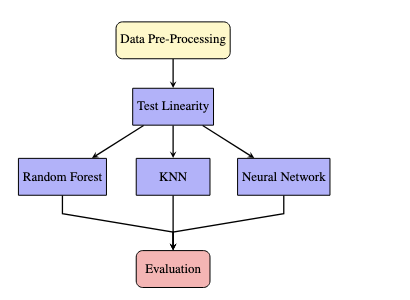
\includegraphics[width=1\linewidth]{pipeline.png} % Ensure the file name is correct
    \caption{Workflow for film revenue classification. Starting with data pre-processing, followed by assessing linear relationships between features and revenue. Three non-linear machine learning models, Random Forest, K-Nearest Neighbors (KNN), and Neural Network, are applied. The models are then evaluated to determine their effectiveness in predicting film revenue.}
    \label{fig:film_revenue_pipeline}
\end{figure}

\subsection{Linearity Test}
To evaluate the initial relationship between individual features and revenue, we performed scatter plot analysis and simple linear regression for interpretable visual and statistical insights. Scatter plots had revenue plotted on the y-axis and each feature on the x-axis to visualize data distribution. Simple linear regression was applied, and the coefficient of determination (\( R^2 \)) was calculated to measure the percentage of variance in revenue explained by each feature.

The predicted revenue (\( \hat{y} \)) was computed using the formula:\[\hat{y} = m \cdot x + c\]
where:
\begin{itemize}
    \item \( m \) (slope) represents the rate of change in revenue for a unit change in the feature:
    \[ m = \frac{\sum{(x - \text{mean}(x)) \cdot (y - \text{mean}(y))}}{\sum{(x - \text{mean}(x))^2}}\]
    \item \( c \) (intercept) is the predicted revenue when the feature value (\( x \)) is zero:\[c = \text{mean}(y) - m \cdot \text{mean}(x)\]
\end{itemize}

The coefficient of determination (\( R^2 \)) was calculated as:
\[R^2 = 1 - \frac{\sum{(y - \hat{y})^2}}{\sum{(y - \text{mean}(y))^2}}\]

An example of pseudocode for generating the plots and \( R^2 \) is as follows:
\begin{algorithm}[H]
\caption{Linearity Validation for Feature and Revenue}\label{alg:linearity}
\KwIn{Dataset with numerical features and revenue}
\KwOut{Combined scatter plots with \( R^2 \) values}
Initialize a combined visualization graph\;

\For{each feature \( x_i \) in features}{ 
    Extract feature \( x_i \) and revenue \( yi \) from the dataset\;
    
    Create a scatter plot of all (\( x_i \), \( yi \)) pairs\;
    
    Annotate the plot with calculated \( R^2 \)\;
}
Save all annotated plots as a combined visualization graph\;
\end{algorithm}

Our analysis of the scatter plots and \( R^2 \) values informed the selection of features for more advanced modeling.

\subsection{Models Application}
Building on the results of the linear regression analysis, we implemented the following machine learning models to capture non-linear relationships and interactions among features:

\subsubsection{Neural Network}
A neural network is a non-linear machine learning model inspired by the human brain that consists of interconnected layers of nodes to learn patterns through training~\hyperref[Hardesty2017]{(Hardesty, 2017)}. Their suitability for revenue prediction lies in two key aspects: 
\begin{enumerate}
    \item The ability to extract abstract representations in hidden layers, enabling them to handle the complexity of multi-class classification.
    \item The capability to handle the large dataset, which supports robust training and enhances the model's capacity to generalize effectively, allowing accurate classification of films into three revenue ranges.
\end{enumerate}
The neural network's performance is evaluated using accuracy and loss plots, while hyperparameters are tuned iteratively to optimize these metrics.

\section{Experiments and Results}
\label{results}
\subsection{Linearity Test}
\subsubsection{Results}

\begin{figure}[H] 
    \centering
    \vspace{0.3cm} 
    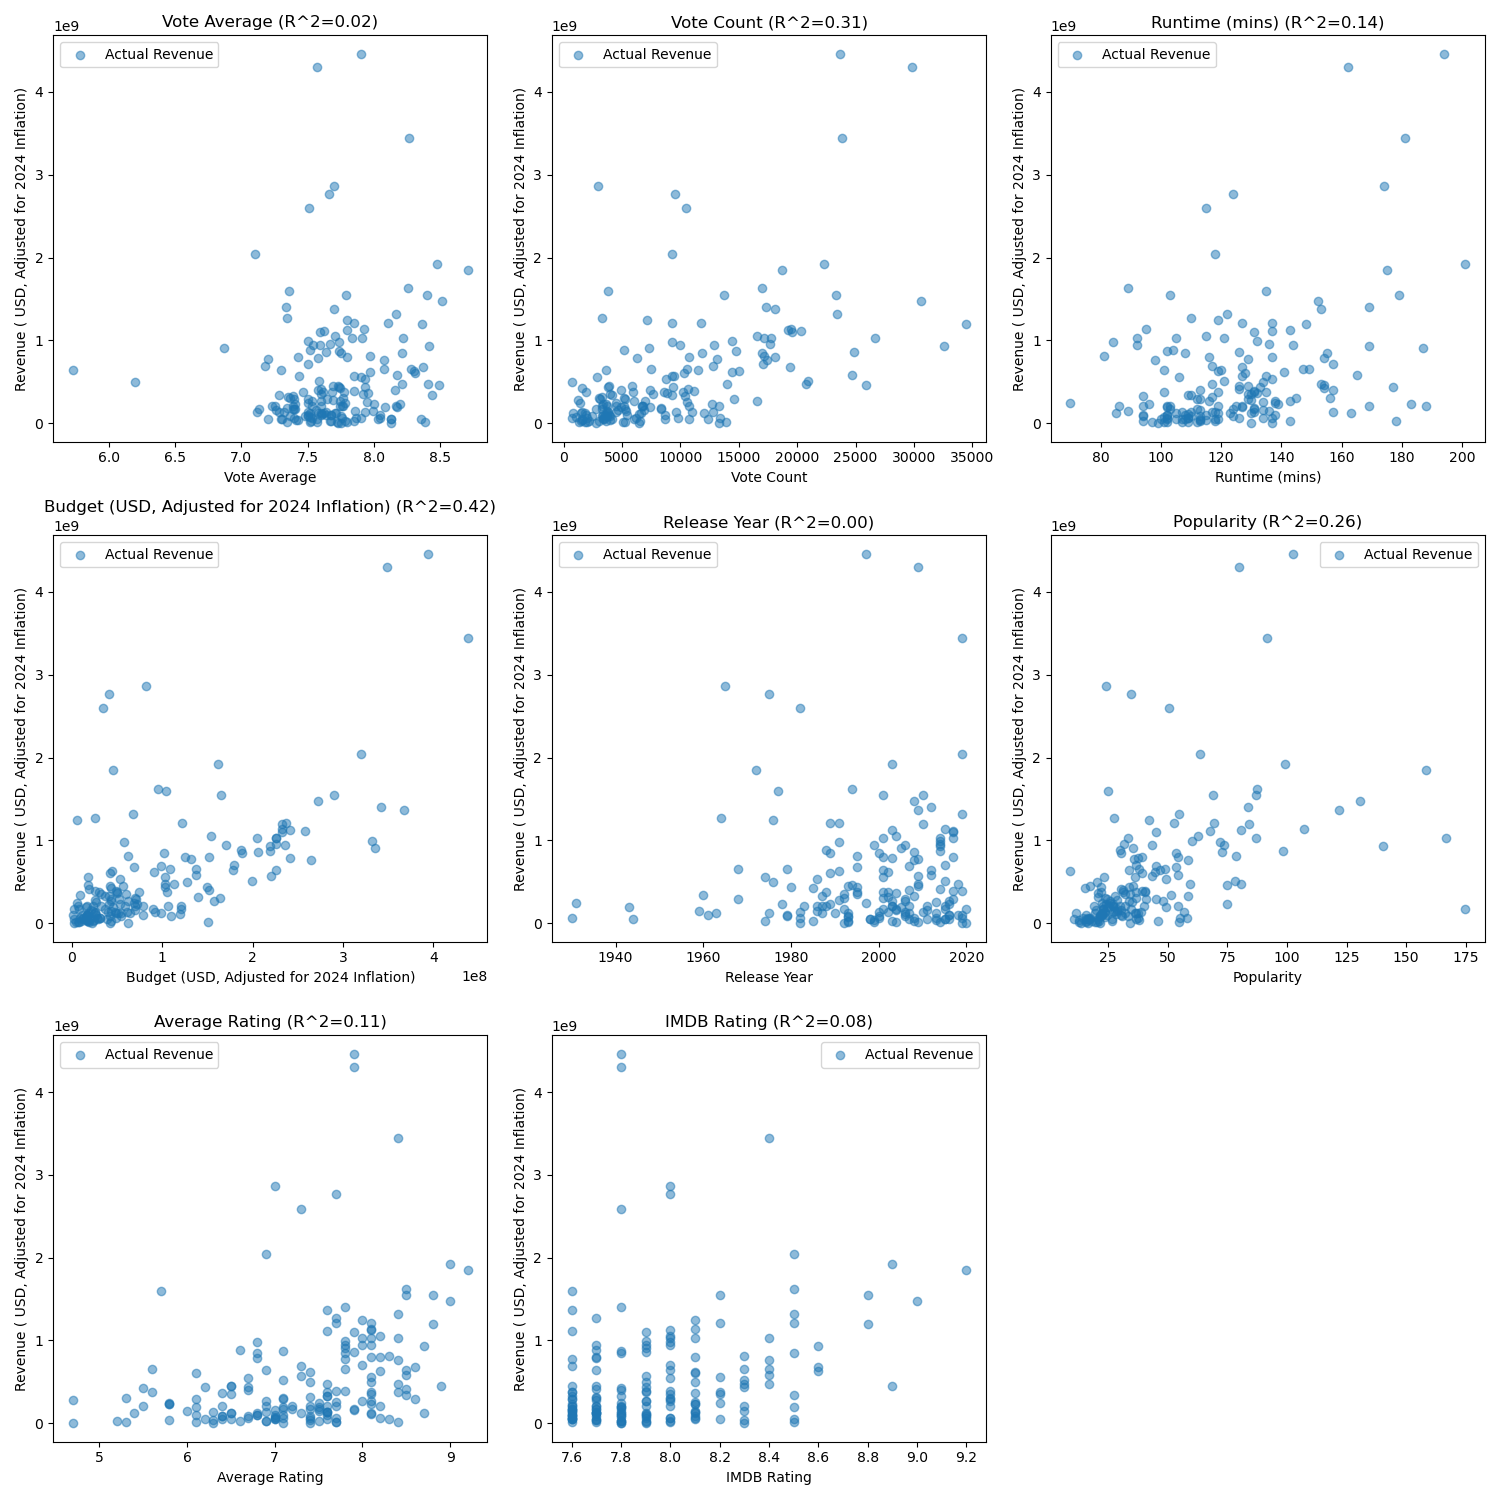
\includegraphics[width=1.1\linewidth]{linear_test.png} % Ensure the file name is correct
    \caption{Scatter plots illustrating the relationship between individual features on the x-axis and revenue on the y-axis. The \( R^2 \) values indicate the strength of linearity. \( R^2 \) values closer to zero indicate weak linear relationships, while \( R^2 \) values closer to one indicate stronger linear relationships. The results demonstrate weak to moderate linear correlations between individual features and revenue.}
    \label{fig:scatter_plots}
\end{figure}

The linearity analysis revealed that no individual feature demonstrates a strong linear relationship with revenue (Fig 1.). Among all features, \textbf{Vote Count} exhibits the strongest linear relationship with revenue from the scatter plot. However, the \( R^2 = 0.31 \) is relatively low, indicating that only a small portion of revenue variance is explained by Vote Count. \textbf{Budget} shows moderate correlation with revenue (\( R^2 = 0.42 \)); however, the scatter suggests significant variability for low-budget films. \textbf{Popularity} (\( R^2 = 0.26 \)) exhibits non-linear patterns for high popularity scores. \textbf{Vote Average} (\( R^2 = 0.02 \)), \textbf{Runtime} (\( R^2 = 0.14 \)), \textbf{Release Year} (\( R^2 = 0.00 \)), \textbf{Average Rating} (\( R^2 = 0.11 \)), and \textbf{IMDb Rating} (\( R^2 = 0.08 \)) showed weak or negligible correlations, with scatter plots indicating non-linear trends (Figure~\ref{fig:scatter_plots}).

\subsubsection{Discussion}
The results suggest that no individual feature exhibits a strong linear relationship with revenue. This finding aligns with previous research highlighting the limitations of linear models for revenue classification, given the non-linear interactions among features \hyperref[SenSharma2021]{(Sen Sharma, et al., 2021)}. Consequently, we concluded that non-linear models are better suited to capture the complex interactions among features and improve revenue classification.
\subsection{Neural Network}
To predict film revenue, a neural network was implemented and trained on the dataset containing over 8,000 samples. 

\subsubsection{Experimental Methodology}

\paragraph{Data Collection and Preprocessing}
Data preprocessing was conducted as detailed in the Method section. All numerical features were normalized and standardized using the \texttt{StandardScaler} to ensure uniform feature scaling. Revenue values were adjusted for 2024 inflation and categorized into \textbf{two} or \textbf{three} classes for classification tasks. For the binary classification task, revenue was divided into:
\begin{itemize}
    \item \textbf{Low}: \( \leq 50,000,000 \)
    \item \textbf{High}: \( > 50,000,000 \)
\end{itemize}
For multi-class classification, revenue was categorized into:
\begin{itemize}
    \item \textbf{Low}: \( \leq 25,000,000 \)
    \item \textbf{Medium}: \( 25,000,000 < \text{revenue} \leq 120,000,000 \)
    \item \textbf{High}: \( > 120,000,000 \)
\end{itemize}
The thresholds for revenue classification were manually selected to ensure a balanced distribution of films across the different classes, thereby enhancing the model's performance on both binary and multi-class classification tasks.

\paragraph{Model Architecture and Training}
A feed-forward neural network with three hidden layers was designed, employing ReLU activation functions, dropout for regularization, and batch normalization to stabilize training. The model was compiled with a stochastic gradient descent (SGD) optimizer and a categorical cross-entropy loss function to handle the multi-class target. A 70/30 train-test split was used for evaluation, and the model was trained for 300 epochs with a batch size of 64.

\paragraph{Evaluation}
Training and validation accuracy were tracked over epochs to monitor convergence and assess the model’s generalization. The final model’s accuracy was evaluated on the validation set, and the classification performance was summarized.

\subsubsection{Result}
\begin{figure}[H] % Keeps the figure at the exact location
    \centering
    \vspace{0.3cm} % Add spacing between the title and figure
    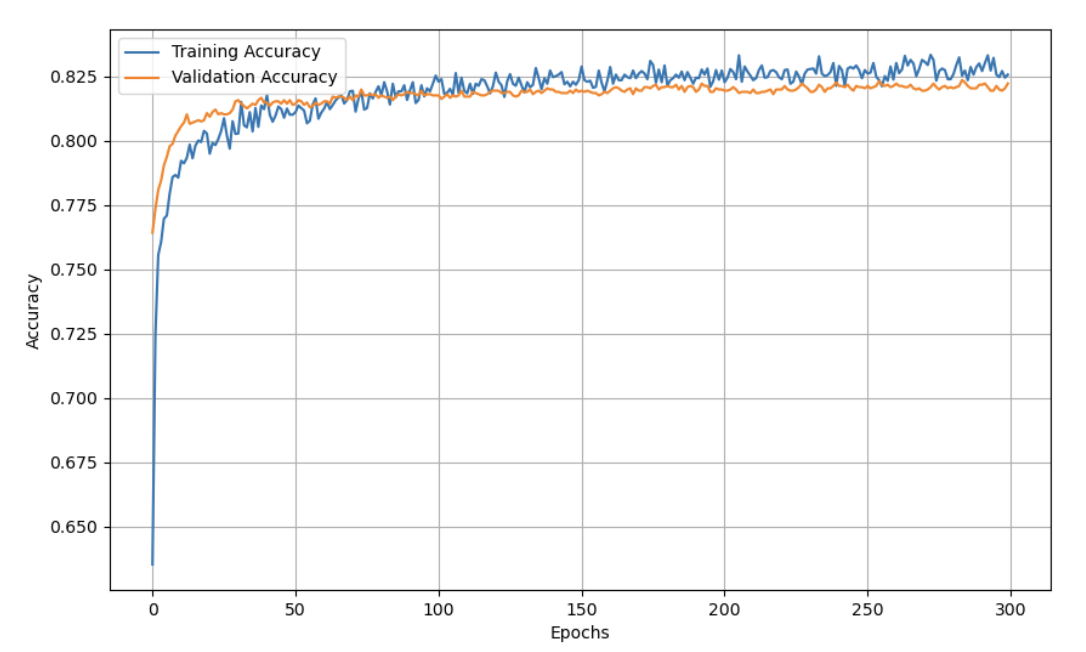
\includegraphics[width=1.0\linewidth]{nn_accuracy.png} % Ensure file is correctly uploaded
    \caption{Training and validation accuracy of the neural network over 300 epochs with 2 revenue classes. The x-axis represents training epochs, and the y-axis represents accuracy. The curves demonstrate consistent convergence, with validation accuracy stabilizing at 82\%, indicating effective generalization.}
    \label{fig:training_validation_accuracy}
\end{figure}

\begin{table}[H]
    \centering
    \small % Reduce font size for the table
    \caption{Classification Report for Neural Network on Film Revenue Classification (Two Classes).}
    \label{tab:classification_report}
    \vspace{0.1in} % Add 0.1 inches of space between the caption and the table
    \begin{tabular}{lccc}
        \toprule
        \textbf{Class} & \textbf{Precision} & \textbf{Recall} & \textbf{F1-Score} \\
        \midrule
        Low Revenue (0)  & 0.81 & 0.83 & 0.82 \\
        High Revenue (1) & 0.83 & 0.82 & 0.82 \\
        \midrule
        \textbf{Accuracy}  & \multicolumn{3}{c}{0.82} \\
        \textbf{Macro Avg} & 0.82 & 0.82 & 0.82 \\
        \textbf{Weighted Avg} & 0.82 & 0.82 & 0.82 \\
        \bottomrule
    \end{tabular}
    \vspace{0.1in} % Add 0.1 inches of space after the table
\end{table}

We observed the following during the training and evaluation of the neural network:

\begin{enumerate}
    \item Both the training and validation accuracy curves showed rapid improvement during the initial epochs, stabilizing around 250 epochs (Figure~\ref{fig:training_validation_accuracy}).
    \item The training accuracy stabilized at approximately 82\%, and the validation accuracy remained close throughout, indicating minimal overfitting (Figure~\ref{fig:training_validation_accuracy}).
    \item The final validation accuracy of 82\% suggests that the neural network effectively captures the non-linear relationships among features (Figure~\ref{fig:training_validation_accuracy}).
    \item The classification report further supports the model's performance. The precision, recall, and F1-scores for all classes are consistent (Precision: 0.81, Recall: 0.83 for Class 0; Precision: 0.83, Recall: 0.82 for Class 1), and the macro-average and weighted-average metrics confirm that the model performs well across all classes, without bias toward any specific revenue range (Table ~\ref{tab:classification_report}).
\end{enumerate}

\begin{table}[H]
    \centering
    \small % Reduce font size for the table
    \caption{Classification Report for Neural Network on Film Revenue Classification (Three Classes).}
    \label{tab:classification_report_three_classes}
    \vspace{0.1in} % Add 0.1 inches of space between the caption and the table
    \begin{tabular}{lccc}
        \toprule
        \textbf{Class} & \textbf{Precision} & \textbf{Recall} & \textbf{F1-Score} \\
        \midrule
        Low Revenue (0)  & 0.80 & 0.75 & 0.77 \\
        Medium Revenue (1) & 0.62 & 0.65 & 0.63 \\
        High Revenue (2) & 0.80 & 0.81 & 0.80 \\
        \midrule
        \textbf{Accuracy}  & \multicolumn{3}{c}{0.73} \\
        \textbf{Macro Avg} & 0.74 & 0.73 & 0.74 \\
        \textbf{Weighted Avg} & 0.74 & 0.73 & 0.73 \\
        \bottomrule
    \end{tabular}
    \vspace{0.1in} % Add 0.1 inches of space after the table
\end{table}

We also ran the neural network for three revenue classes and received lower accuracy and higher variability. Neural network achieves higher overall accuracy (82\%) in the binary classification compared to 73\% in three-class classification. The three-class classification also exhibits moderate precision and recall variability compared to binary class classification. In Table 2., the middle revenue range (Class 1) achieves Precision 0.62 and Recall 0.65, which are notably lower compared to the high (Class 2: Precision 0.80, Recall 0.81) and the low revenue range (Class 0: Precision 0.80, Recall 0.75) (Table ~\ref{tab:classification_report_three_classes}). These results highlight the model failed to classify the middle revenue class compared to the other classes.

\subsubsection{Discussion}

The results demonstrate that the neural network effectively models the complex interactions among features, achieving \textbf{82\% accuracy} and balanced performance for two revenue classes, outperforming linear models. This highlights the model’s robustness in handling varying data distributions. The close alignment of training and validation curves further underscores the model's ability to generalize effectively.

For the three-class revenue classification, the neural network achieved a lower overall accuracy of \textbf{73\%}, with greater variability. This variability is expected due to the middle revenue range often sharing characteristics with low- and high-revenue films. The additional complexity also makes it challenging for the neural network to accurately model the boundaries between classes.

Overall, the neural network demonstrates strong performance, with better accuracy and more consistent results in the two-class scenario due to the more distinct separation of classes. However, the specific features contributing most to the classification remain unclear, as the neural network operates as a black-box model.

\section{Conclusions}
\label{conclusion}

Lessons learned.  Wrap up the paper with a restatement of the initial hypothesis
and your findings.  Discuss unanswered questions/possible future work to further
the study of this central question.

\section{Social impact}
\label{conclusion}

Lessons learned.  Wrap up the paper with a restatement of the initial hypothesis
and your findings.  Discuss unanswered questions/possible future work to further
the study of this central question.

\section*{Acknowledgments}


Place acknowledgements in an unnumbered section at the
end of the paper. Typically, this will include
to colleagues who contributed to the ideas, individuals who
reviewed your submission, or external sources who helped
acquire data.

\section*{references}
\begin{hangparas}{.25in}{1} % Set hanging indent of 0.25in
\hypertarget{Hardesty2017}{Hardesty, L. Explained: Neural Networks. \textit{MIT News Office}. Archived on 18 March 2024. Retrieved on 2 June 2022, 14 April 2017.}
\end{hangparas}
\begin{hangparas}{.25in}{1}
\hypertarget{SenSharma2021}{Sen Sharma, A., Roy, T., Rifat, S. A., \& Mridul, M. A. Presenting a Larger Up-to-date Movie Dataset and Investigating the Effects of Pre-released Attributes on Gross Revenue. \textit{arXiv preprint}, arXiv:2110.07039 [cs.IR], 13 October 2021. \url{https://arxiv.org/abs/2110.07039}}

\end{hangparas}


\bibliographystyle{icml2014}

\end{document}


% This document was modified from the file originally made available by
% Pat Langley and Andrea Danyluk for ICML-2K. This version was
% created by Lise Getoor and Tobias Scheffer, it was slightly modified
% from the 2010 version by Thorsten Joachims & Johannes Fuernkranz,
% slightly modified from the 2009 version by Kiri Wagstaff and
% Sam Roweis's 2008 version, which is slightly modified from
% Prasad Tadepalli's 2007 version which is a lightly
% changed version of the previous year's version by Andrew Moore,
% which was in turn edited from those of Kristian Kersting and
% Codrina Lauth. Alex Smola contributed to the algorithmic style files.



\usepackage{tikz}
\usetikzlibrary{shapes.geometric, arrows}

\tikzstyle{startstop} = [rectangle, rounded corners, minimum width=2cm, minimum height=1cm, text centered, draw=black, fill=red!30]
\tikzstyle{process} = [rectangle, minimum width=2cm, minimum height=1cm, text centered, draw=black, fill=blue!30]
\tikzstyle{decision} = [rectangle, rounded corners, minimum width=2cm, minimum height=1cm, text centered, draw=black, fill=yellow!30]
\tikzstyle{arrow} = [thick,->,>=stealth]



\begin{tikzpicture}[node distance=2cm, scale=0.8, every node/.style={transform shape}]

% Nodes
\node (dataprocessing) [decision] {Data Pre-Processing};
\node (linearity) [process, below of=dataprocessing, yshift=0.2cm] {Test Linearity};
\node (rf) [process, below of=linearity, xshift=-3cm, yshift=0.1cm] {Random Forest};
\node (knn) [process, below of=linearity, yshift=0.1cm] {KNN};
\node (nn) [process, below of=linearity, xshift=3cm, yshift=0.1cm] {Neural Network};
\node (evaluation) [startstop, below of=knn, yshift=-0.5cm] {Evaluation};

% Arrows
\draw [arrow] (dataprocessing) -- (linearity);
\draw [arrow] (linearity) -- (rf);
\draw [arrow] (linearity) -- (knn);
\draw [arrow] (linearity) -- (nn);
\draw [arrow] (rf) -- ++(0,-1) -- ++(3,-0.5) -- (evaluation);
\draw [arrow] (knn) -- (evaluation);
\draw [arrow] (nn) -- ++(0,-1) -- ++(-3,-0.5) -- (evaluation);